\documentclass{article}
\usepackage{graphicx}
\begin{document}
\hfill Alejandro Chavez

\hfill Digital Logic

\hfill \today\\

\begin{center}\begin{large}Lab 5\end{large}\end{center}
  Part 1
\begin{itemize}
	\item
  1) Register Transfer Circuit\\
  \linebreak
  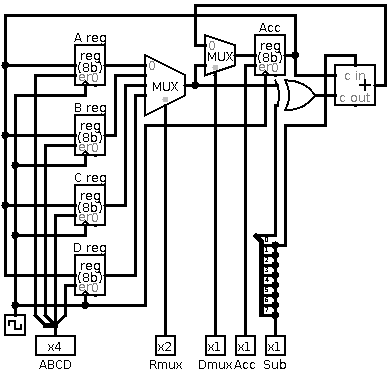
\includegraphics[scale=0.5]{Lab5_part1.png}\\
  2)\\
  There are 9 bits in the control code.
\end{itemize}
	Part 2 - Coding your Register Transfer Sequence
\begin{itemize}
	\item
    1)
  \begin{itemize}
    \item
      1)\\
      $A\to Acc$
    \item
      2)\\
      $Add(Acc, B)\to Acc$
    \item
      3)\\
      $Sub(Acc, C)\to Acc$
    \item
      4)\\
      $Add(Acc, D)\to Acc$
  \end{itemize}
  \item
    2)
  \begin{itemize}
    \item
      1)\\
      $A\to Acc$\\
      $000000110$
    \item
      2)\\
      $Add(Acc, B)\to Acc$\\
      $000001010$
    \item
      3)\\
      $Sub(Acc, C)\to Acc$\\
      $000010011$
    \item
      4)\\
      $Add(Acc, D)\to Acc$\\
      $000011010$
  \end{itemize}
  \item
    3)
  \begin{itemize}
    \item
      1)\\
      $0x13 = 19_{10}$
    \item
      2)\\
      $0x5B = 91_{10}$
    \item
      3)\\
      $0x3A = 58_{10}$
    \item
      4)\\
      $0xF0 = 240_{10}$
  \end{itemize}
  \item
    4)
  \begin{itemize}
    \item
      1)\\
      $A\to Acc$\\
      $Acc=0x13=19$
    \item
      2)\\
      $Add(Acc, B)\to Acc$\\
      $Acc=19+91=110=0x6E$
    \item
      3)\\
      $Sub(Acc, C)\to Acc$\\
      $Acc=110-58=52=0x34$
    \item
      4)\\
      $Add(Acc, D)\to Acc$\\
      $Acc=52-16=36=0x24$
  \end{itemize}
  \item
    5)\\
    None of the operations produced overflow.
  \item
    6)\\
    $0x24=36$
  \item
    7)\\
    $(((A+B)-C)+D)$
\end{itemize}
	Part 3 - Executing and Recording You Register Transfer Sequence
\begin{itemize}
	\item
  1) Execution Trace Table\\

  \begin{tabular}{c|ccccc|c|c}
    Time & A       & B      & C      & D      & Acc    & Control Code & Action \\ \hline
    $0$  & $0x13$  & $0x5B$ & $0x3A$ & $0xF0$ & $0x00$ & $0000$ $00$ $1$  $1$  $0$ & $A\to Acc$ \\
    $1$  & $0x13$  & $0x5B$ & $0x3A$ & $0xF0$ & $0x13$ & $0000$ $01$ $0$  $1$  $0$ & $Add(B, Acc)\to Acc$ \\
    $2$  & $0x13$  & $0x5B$ & $0x3A$ & $0xF0$ & $0x6E$ & $0000$ $10$ $0$  $1$  $1$ & $Sub(C, Acc)\to Acc$ \\
    $3$  & $0x13$  & $0x5B$ & $0x3A$ & $0xF0$ & $0x34$ & $0000$ $11$ $0$  $1$  $0$ & $Add(D, Acc)\to Acc$ \\
    $4$  &         &        &        &        & $0x24$ &                           &                      \\
  \end{tabular}\\

  There should be 5 registers.
\end{itemize}
\end{document}
